\section{Rețele neuronale convoluționale (CNNs)}

Motivația din spatele acestor tipuri de rețele a apărut atunci când cercetătorii au încercat să aplice tehnicile clasice de deep learning în domeniul computer vision. Cel mai mare impediment a fost lipsa puterii computaționale. Spre exemplu, pentru o imagine RGB cu dimensiunile 32x32x3 avem un vector de intrare cu $3072$ de componente, iar dacă primul layer din rețea are $3500$ de neuroni, prima matrice de parametri va avea forma $(3500, 3072)$, adică peste 10 milioane de parametrii de optimizat numai pentru primul layer. Este evident faptul că, pentru ca deep learning să fie aplicat în recunoașterea imaginilor, ne trebuie o altă abordare.

\subsection{Operația de convoluție}
Fie 2 matrici, $I$ matricea de pixeli corespunzătoare unei imagini și $K$ o matrice $kernel (filter)$. Operația de convoluție având ca termeni $I$ și $K$ arată în felul următor:

\begin{center}
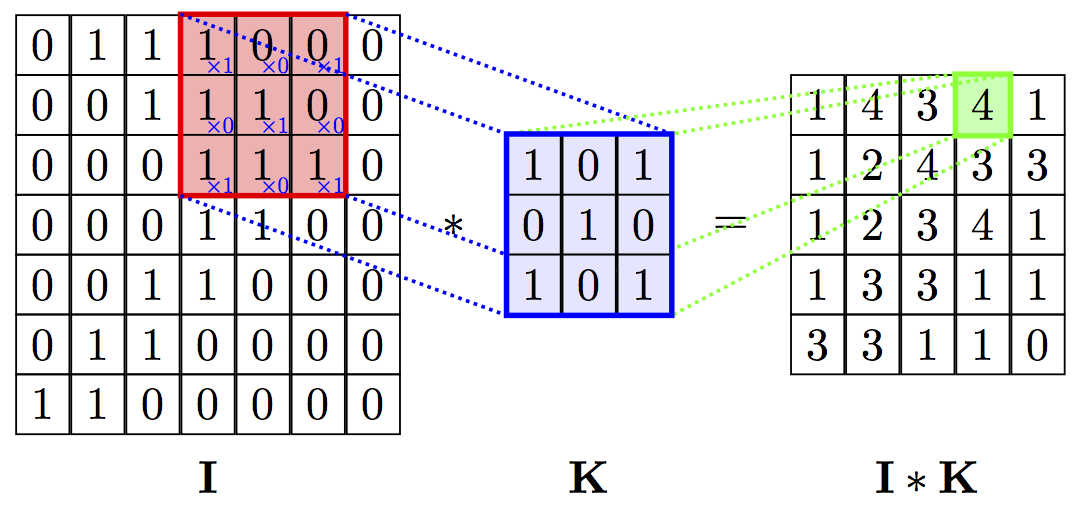
\includegraphics[scale=1.5]{convolution} \\
\textit{Fie I de forma (n,n) și K de forma (f,f). Matricea rezultat va avea forma (n-f+1,n-f+1)}
\end{center}


\subsubsection{Padding și Striding}
Padding-ul a venit ca o soluție pentru cazul în care filter-ul iese în afara imaginii în aproprierea marginilor acesteia. Astfel, se va completa matricea inițială cu zero-uri înaintea efectuării operației propriu-zise.

\begin{center}
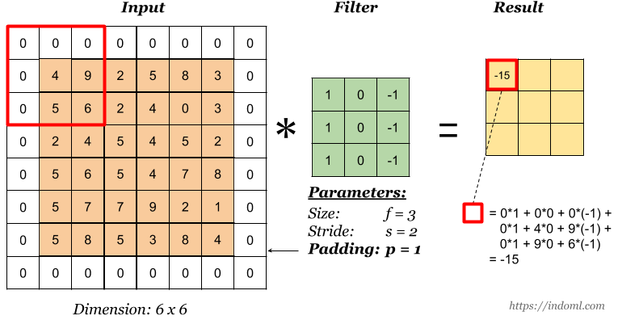
\includegraphics[scale=0.7]{padding}
\end{center}

Această tehnică modifică regula dimensiunii output-ului. Pentru un padding de dimensiune $p$ vom aveaun output de forma $(n+2p-f+1, n+2p-f+1)$. Observăm că operația de convoluție clasică (fără padding) micșorează imaginea, însă, dacă vrem să evitam acest lucru, putem alege un padding $\displaystyle{p=\frac{f-1}{2}}$.

Stridding-ul se referă la numărul de unități cu care vom mișca filter-ul pentru a scana întreaga imagine. Până acum am folosit un stride $s=1$.

\begin{center}
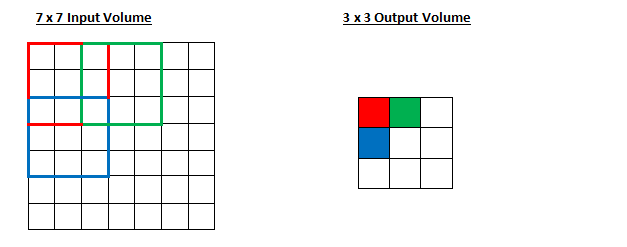
\includegraphics[scale=1]{stride} \\
\textit{Operație de convoluție cu stride-ul s = 2}
\end{center}

Scopul acestei tehnici este să reducă numărul de operații având ca compromis, o mică pierdere de informație. Astfel output-ul obținut va avea forma $\displaystyle{\left(\displaystyle{\left[\frac{n+2p-f}{s}\right]}+1, \displaystyle{\left[\frac{n+2p-f}{s}\right]}+1\right)}$.

\subsubsection{Convoluție peste volume}

Deocamdată, am vorbit despre operația de convoluție pe matrici de pixeli de forma $(n,m)$ ce reprezintă imagini $greyscale$. În contextul imaginilor RGB, matricile lor au forma $(n,m,3)$, iar pentru a putea efectua operația, vom copia filter-ul de 3 ori, formând o matrice de forma $(f,f,3)$. Pentru fiecare channel, vom lua filter-ul si vom face calculele ca înainte, obtinând 3 numere pentru fiecare poziție din output. La final vom aduna aceste 3 numere pentru a calcula o componentă a output-ului, forma acestuia rămânând aceeași ca în cazul imaginilor cu un singur channel.

\begin{center}
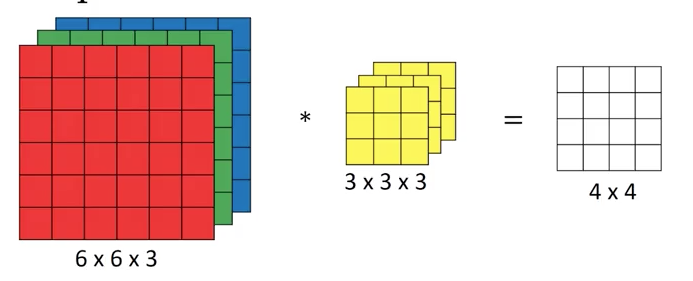
\includegraphics[scale=0.4]{convVolumes} \\
\end{center}

După ce am studiat ce este un filter și operația de convoluție, putem defini un layer într-o rețea neuronală convoluțională ca o multitudine de filtere și de operații de convoluție efectuate pe o matrice de pixeli. Aceste operații sunt independente, însă output-ul lor este combinat la final în următorul mod:

\begin{center}
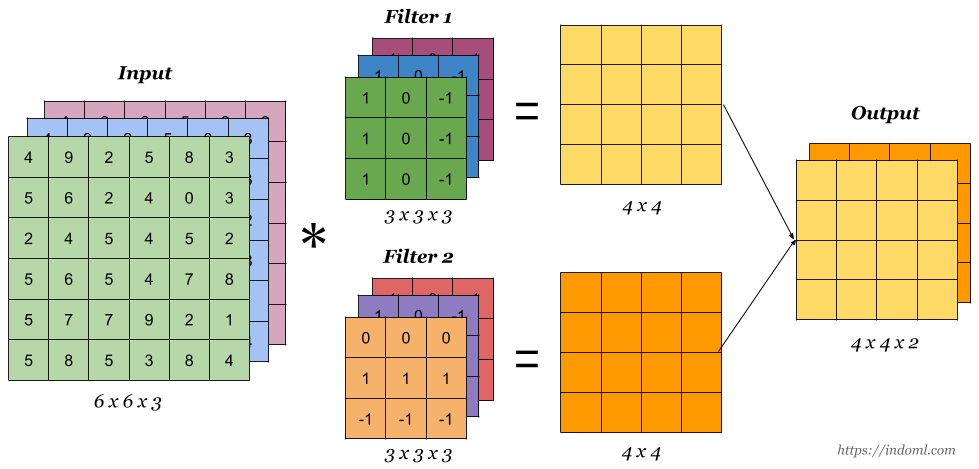
\includegraphics[scale=0.4]{convLayer} \\
\textit{Un layer cu 2 filtere}
\end{center}

Vom compara această abordare cu cea a rețelelor neuronale clasice. Având 2 filtere, vom lua cazul clasic a unui layer cu 2 neuroni obișnuiți. În contextul clasic, având un input de forma $(6,6,3)$ și 2 neuroni, matricea de parametrii va avea forma $(2,6*6*3)$, în total 216 de parametrii. În cazul rețelelor convoluționale, avem 2 filtere de forma $(3,3,3)$, în total 54 de parametrii, făcând aceste rețele mult mai viabile pentru prelucrarea imaginilor de rezoluție înaltă.

\subsubsection{Max pooling}
Max pooling este un pas intermediar efectuat între layer-ele de convoluție, în special pentru a reduce dimensiunea vectorilor și complexitatea calculelor. Ca și în cazul operației de convoluție, max pooling are 3 hyperparametrii $(filterSize \, f, padding \, p ,stride \, s)$ și formula formei output-ului este aceeași $\displaystyle{\left(\displaystyle{\left[\frac{n+2p-f}{s}\right]}+1, \displaystyle{\left[\frac{n+2p-f}{s}\right]}+1\right)}$.
 
\begin{center}
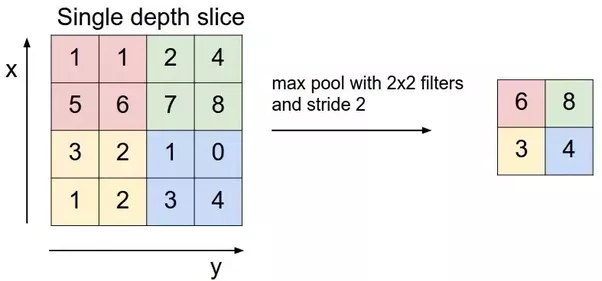
\includegraphics[scale=0.5]{maxPooling}
\end{center}

Este de observat că, spre deosebire de un layer obișnuit, cel de max pooling nu prezintă parametrii ce trebuie învățați, fiind o funcție fixată. În literatura de specialitate mai este întâlnit și $Average Pooling$ în care nu luăm componenta maximă, ci facem media tuturor componentelor.

\subsection{Arhitecturi celebre}
O rețea neuronală convoluțională este o succesiune de layere de convoluție, intercalate de cele de max pooling. În practică este greu să găsim o configurație a acestor layere care să ofere cea mai bună performanță. Din această cauză, un punct bun de plecare este reprezentat de arhitecturile celebre consacrate in literatura de specialitate.

\subsubsection{LeNet-5}
LeNet-5 a fost prima rețea neuronală convoluțională cu rezultate notabile și folosită în afara unor experimente. Ea a fost folosită în anii 90 cu succes la recunoașterea cifrelor și a literelor de mână date ca input sub forma unei imagini RGB de rezoluție 32x32. Mai jos este arhitectura rețelei cu detalii despre hyperparametrii. \cite{lenet}

\begin{center}
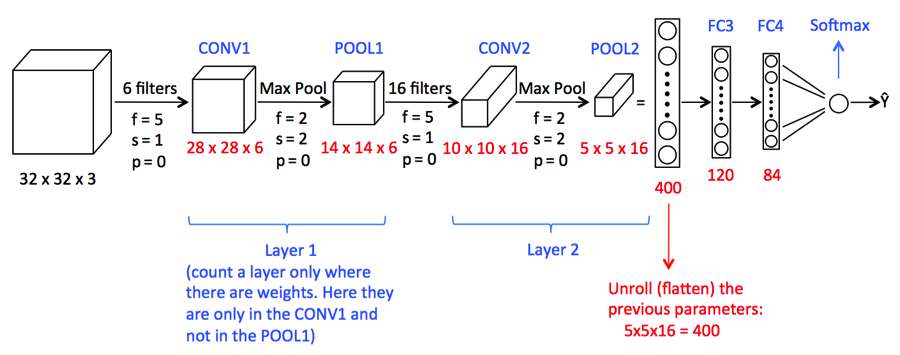
\includegraphics[scale=0.5]{LeNet5}
\end{center}

\subsubsection{AlexNet}
AlexNet este una dintre cele mai importante rețele neuronale convoluționale deoarece, în anul 2012, a reușit să aducă rata de eroare în cadrul competiției ImageNet LSVRC-2010 de la 25\% la 16\%, deschizând drumul tehnicilor de deep learning în domeniul Computer Vision. Arhitectura folosită este asemănătoare rețelei LeNet-5, folosind tot o secvență liniară de layere convoluționale intercalate cu cele de max pooling. \cite{alexnet}

\begin{center}
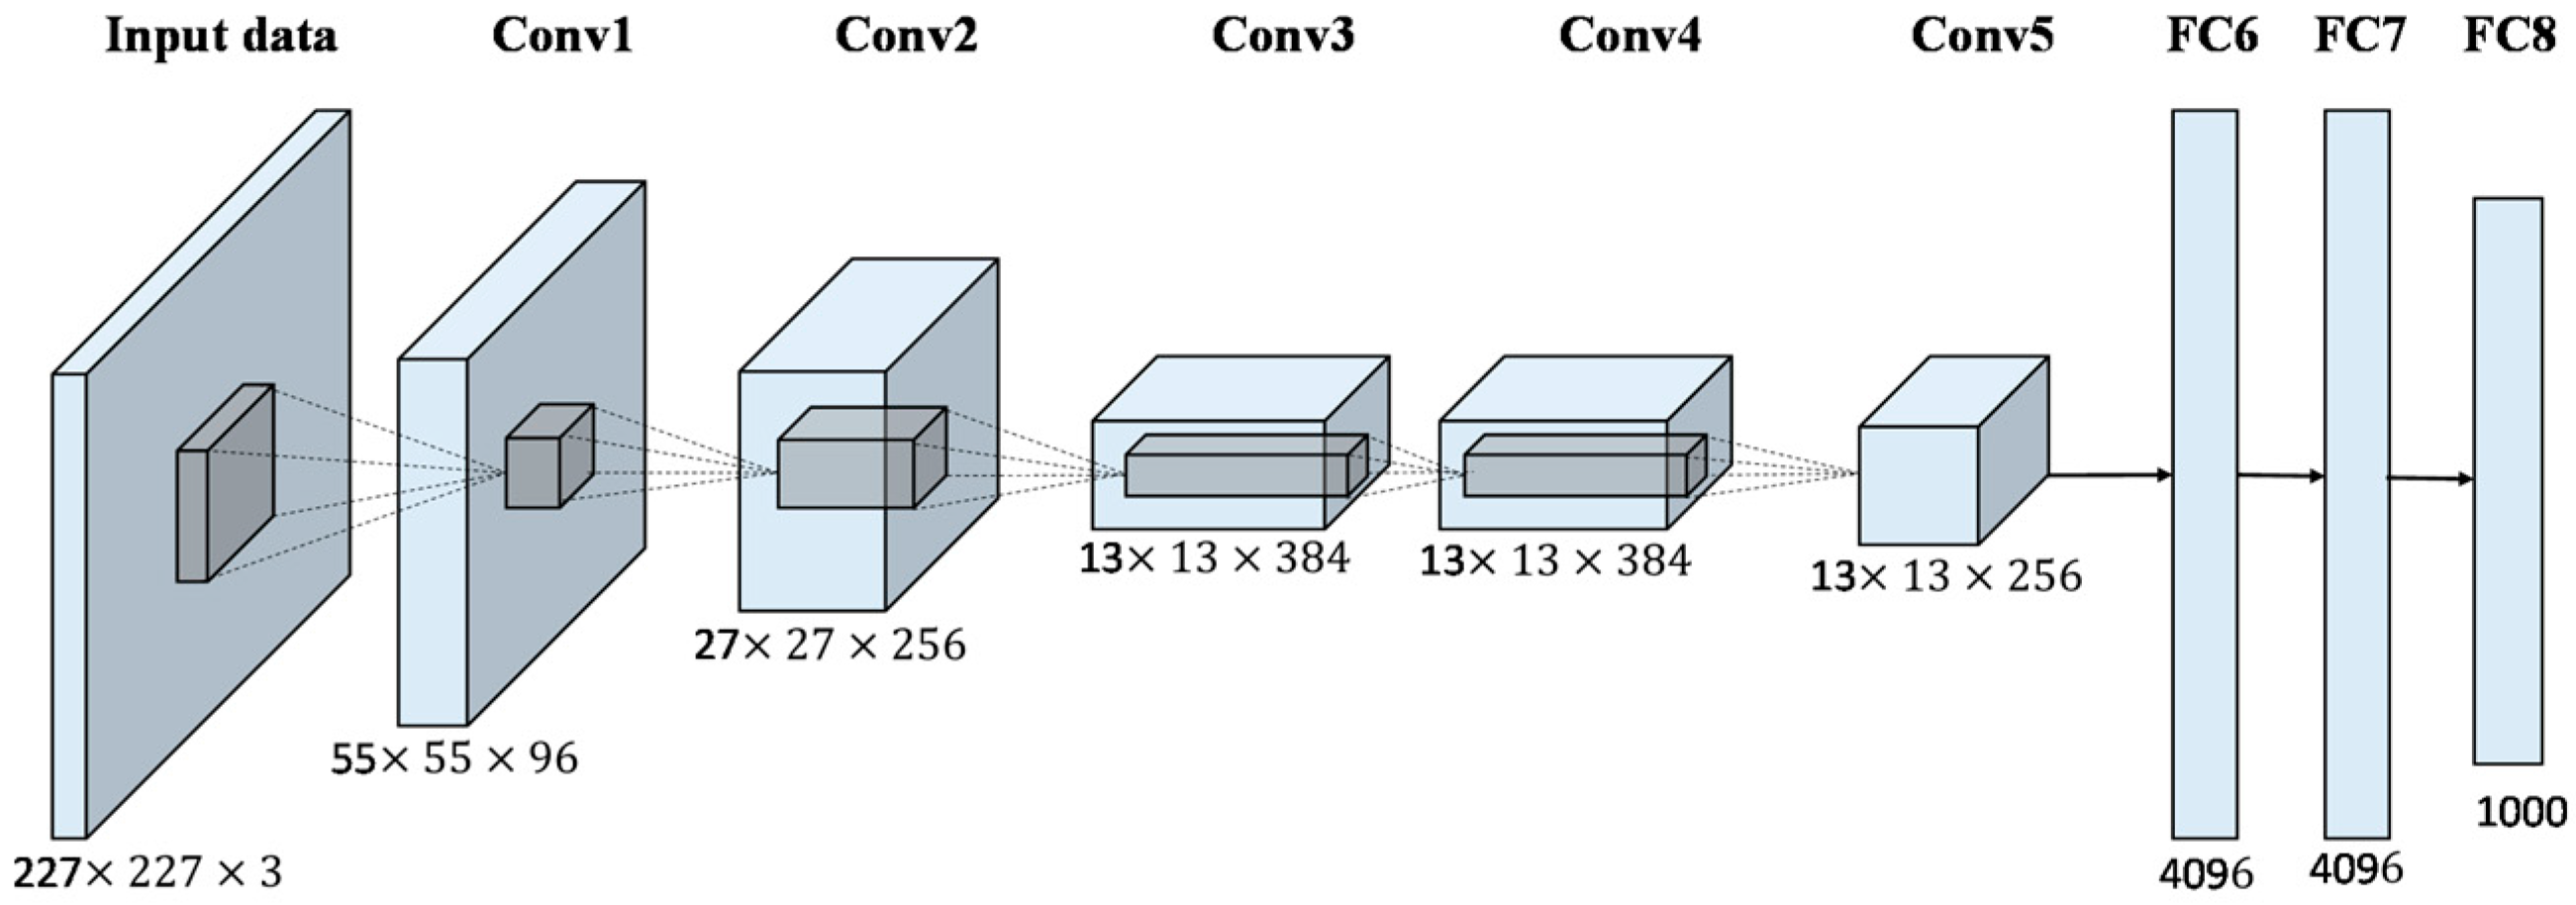
\includegraphics[scale=1.5]{alexnet}
\end{center}

\subsubsection{VGG-16}
Această rețea a fost creată de $Visual \; Geometry \; Group$ din cadrul universității Oxford în anul 2014. VGG-16 a obținut rezultate foarte bune în cadrul competiției ImageNet LSVRC-2010, reușind să depășească performanța oferită de AlexNet. Rețeaua a ieșit în evidență prin numărul foarte mare de parametrii ce erau învățați ($\approx 100 \, mil$), acesta fiind și principalul motiv pentru îmbunătățirile aduse. \cite{vgg16}

\begin{center}
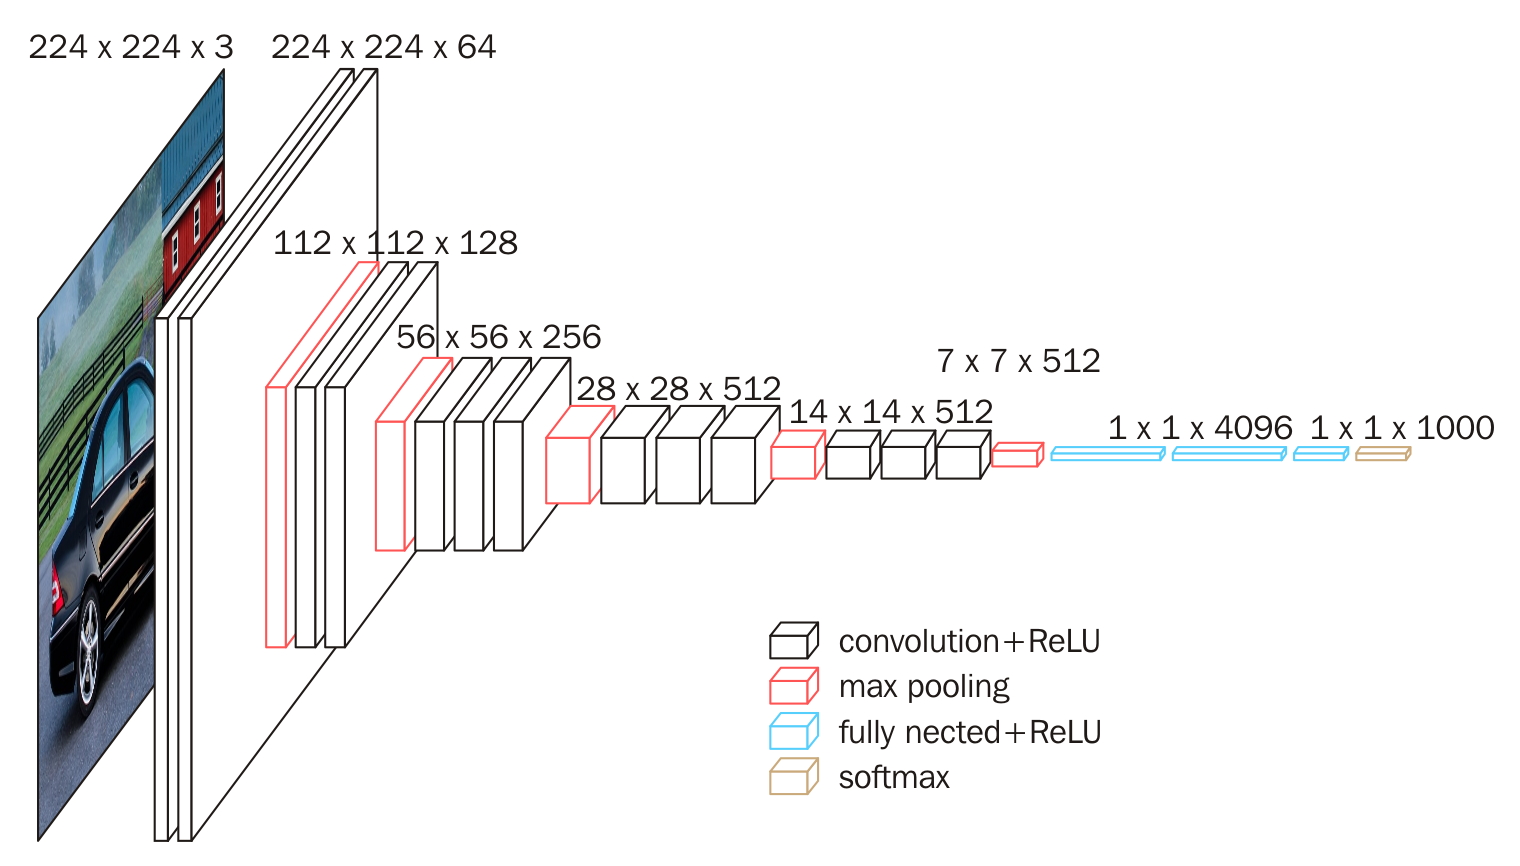
\includegraphics[scale=1]{vgg16} \\
\textit{Arhitectura VGG-16}
\end{center}

\subsubsection{ResNet}
Modelul ResNet a fost introdus în 2015 de cei de la Microsoft și ideea din spate este foarte simplă: \textit{Deeper is better}. Văzând îmbunătățirile aduse din VGG-16 prin simplul fapt că avea foarte mulți parametrii, cercetătorii care au creat ResNet au dorit să creeze o rețea cât mai mare în adâncime cu speranța că performanța va crește. O mare problemă a fost complexitatea calculelor pentru antrenarea unei astfel de rețele, fiind necesar să recurgă la o tehnică numită $Residual \; learning \; block$ pe care o vom descrie imediat. Asrfel, ResNet a putut fi antrenat, având diferite variante, în funcție de numărul de layere: ResNet-34, ResNet-50, ResNet-152. \cite{resnet}

\begin{center}
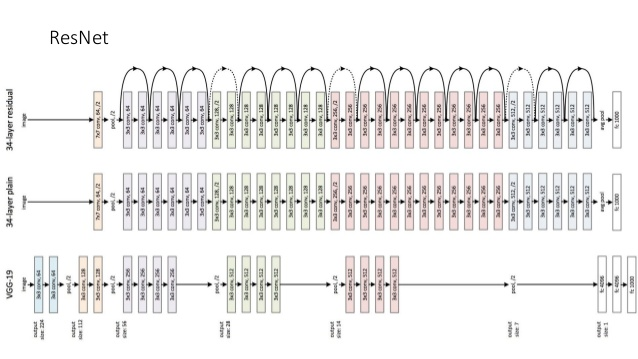
\includegraphics[scale=0.5]{resnet} \\
\textit{ResNet-34 (sus) în comparație cu un CNN obișnuit și cu VGG-19 (o variantă extinsă a VGG-16)}
\end{center}

\begin{center}
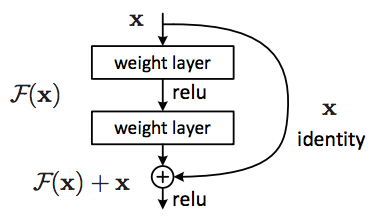
\includegraphics[scale=0.7]{residualBlock} \\
\textit{Residual Block}
\end{center}

Acest bloc este, în mare parte, o construcție obișnuită dintr-un CNN, exceptând acea conecțiune (skip connection) ce sare cele 2 layere. La un nivel înalt, având o înșiruire de blocuri de acest tip, orice layer ce nu aduce informații utile, poate fi evitat, fiind foarte ușor pentru un algoritm de tipul \textit{Gradient Descent} să învețe funcția identitate într-un astfel de context. Datorită acestui fapt, putem crea rețele neuronale convoluționale cu peste 150 de layere și procesul de antrenament să rămână viabil în continuare.

\subsubsection{Inception}
Dacă cei de la Microsoft au mers pe ideea crearii unei rețele cu foarte multe layere, în 2014, cei de la Google au propus o extindere a modelului clasic prin mărimea lățimii rețelei, construind ceea ce se numește în literatura de specialitate \textit{Inception Block}.

\begin{center}
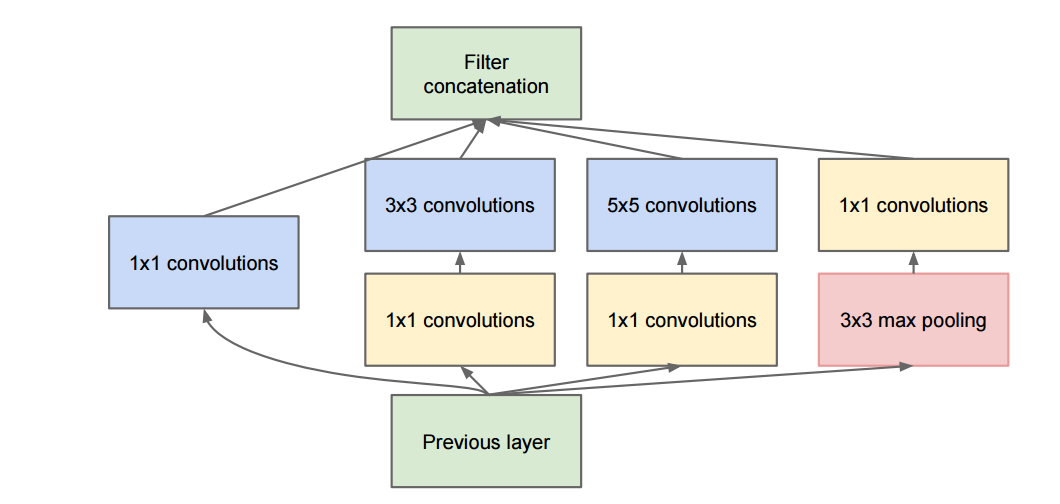
\includegraphics[scale=0.4]{inceptionBlock} \\
\textit{Inception Block}
\end{center}

Principiul de bază este următorul:

\begin{itemize}
\item La un moment dat în construcția arhitecturii putem să alegem dintr-o mulțime de operații (convolutie cu un filter de forma 1x1, cu un filter de forma 3x3, max pooling, etc...) și este dificil să stim anterior care ne aduce performanța cea mai bună. Într-un Inception Block se efectuează toate aceste operații și se concateneaza output-ul la final.
\end{itemize} 

O secventă în cascadă de Inception Blocks reprezintă o rețea convoluțională de tip Inception. \cite{inception}

\begin{center}
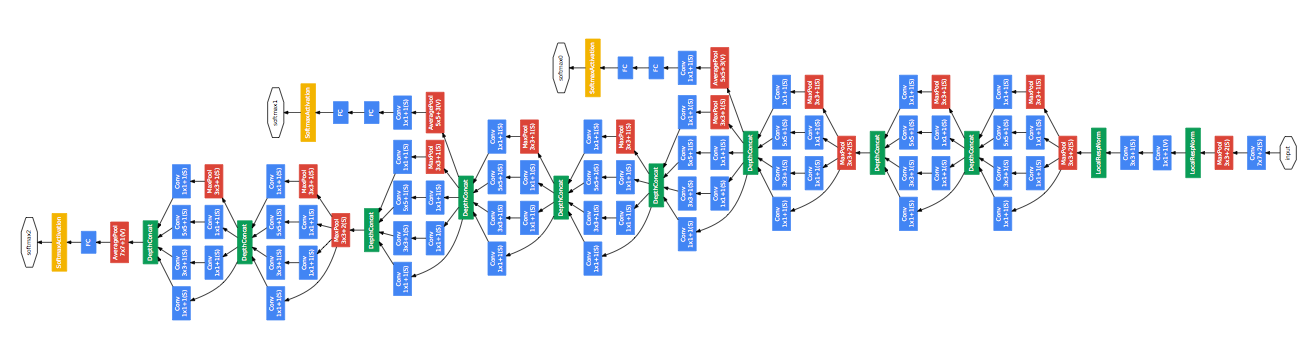
\includegraphics[scale=0.7]{inception}
\end{center}

Diferite modificări au fost aduse acestui model, cel din 2014 purtând numele de Inception-V1, iar acum existând și Inception-V4.

\subsubsection{Xception}
Francois Chollet aduce îmbunătățiri în anul 2016 modelului ResNet, construind o rețea cu conecțiuni reziduale, dar în care înlocuiește toate operațiile de convoluție clasice din layere, cu operații numite \textit{Deapthwise Separable Convolution}. \cite{xception}

\begin{center}
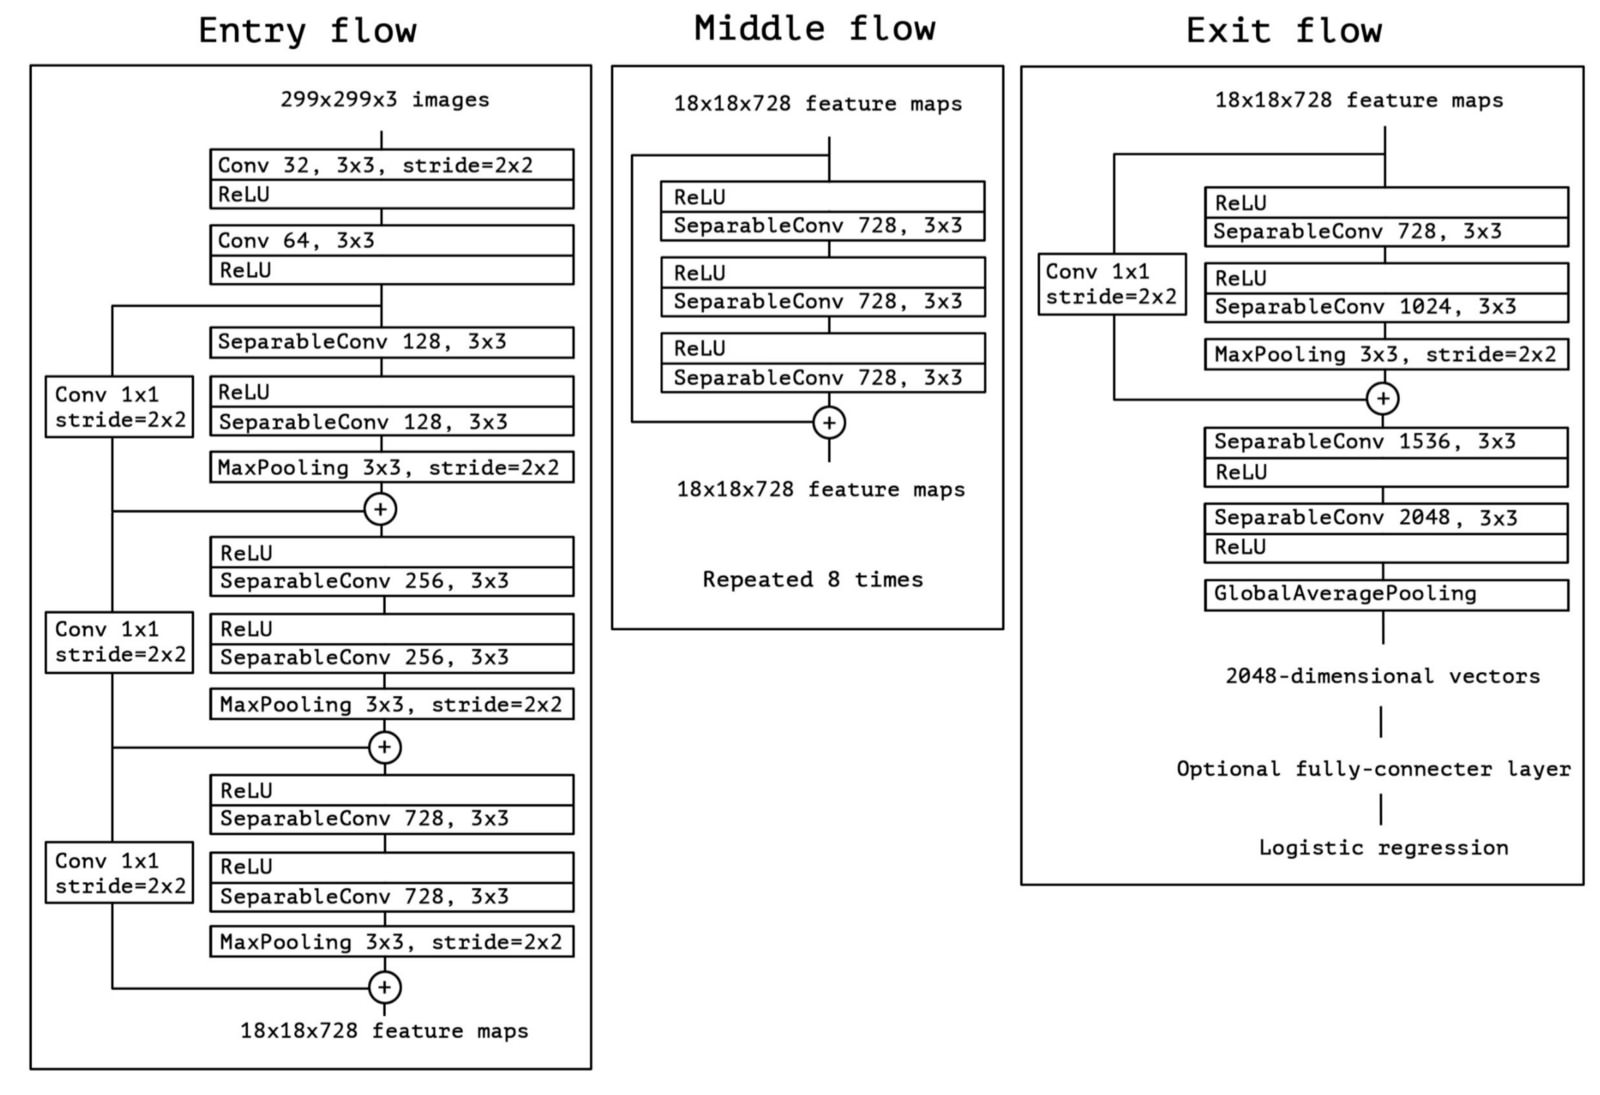
\includegraphics[scale=0.3]{xception}
\textit{Arhitectura rețelei Xception}
\end{center}

Deapthwise Separable Convolution împarte operația clasică în două. De exemplu, dacă avem o imagine I de forma $(n,m,3)$ și un filter de forma $(f,f,3)$, în loc să facem operația pe aceste blocuri, mai întai o vom face pe I cu un nou filter de forma $(f,f,1)$, urmând să aplicăm un al doilea filter de forma $(1,1,3)$ pe rezultatul obținut în pasul precedent. Observăm că forma output-ului se păstrează, în schimb scad de $\approx$ 9 ori numărul de înmulțiri de efectuat și numărul de parametrii ce trebuie învățați.

\begin{center}
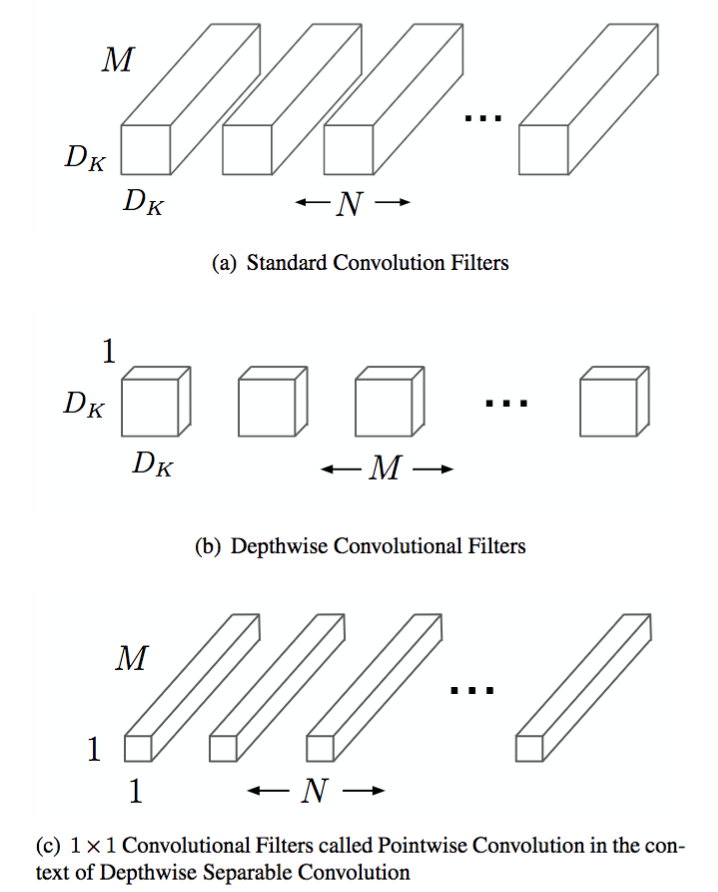
\includegraphics[scale=0.4]{depthconv}
\end{center}

\subsection{Transfer Learning}
Transfer learning se referă la faptul că nu tot ce a învățăt o rețea neuronală pentru o anumită problemă devine inutil când vrem să-i dăm aceleași rețele o nouă problemă. Neavând resurse computaționale foarte mari, această tehnică este o componentă esențială în cadrul proiectului meu. Astfel, folosind un model deja antrenat (Xception) pe datele din competiția ImageNet LSVRC-2010, am extras vectori caracteristici pentru fiecare imagine din setul meu de date, nemaiantrenând modelul. Am avut succes deoarece imaginile din cadrul ImageNet, majoritatea fiind obiecte obișnuite din jurul nostru, nu diferă foarte mult de ceea ce se găsește într-o fotografie făcută într-un restaurant. Ar fi fost imposibil pentru mine să o iau de la 0, ținând cont că modelele descrise anterior au fost antrenate în cloud, chiar și timp de câteva săptămâni fără oprire.